\documentclass{beamer}
%
% Choose how your presentation looks.
%
% For more themes, color themes and font themes, see:
% http://deic.uab.es/~iblanes/beamer_gallery/index_by_theme.html
%
\mode<presentation>
{
  \usetheme{Boadilla}      % or try Darmstadt, Madrid, Warsaw, ...
  \usecolortheme{beaver} % or try albatross, beaver, crane, ...
  \usefonttheme{default}  % or try serif, structurebold, ...
  \setbeamertemplate{navigation symbols}{}
  \setbeamertemplate{caption}[numbered]
  
} 

\usepackage{xcolor,colortbl}
\usepackage[english]{babel}
\usepackage[utf8x]{inputenc}
\usepackage{courier}
\usepackage{dsfont}
\usepackage{verbatim} 
\usepackage{enumerate}
\usepackage{tikz}
\usepackage{multirow}
\usepackage{venndiagram}
\usepackage{epigraph} 
%\usepackage{xcolor}
\usepackage{makecell}

%\usepackage{enumitem}

\usepackage{hyperref}
\hypersetup{
    colorlinks=true,
    linkcolor=blue,
    filecolor=magenta,      
    urlcolor=cyan,
}

% R stuff!
\usepackage{listings}
\definecolor{codegreen}{rgb}{0,0.6,0}
\definecolor{codegray}{rgb}{0.5,0.5,0.5}
\definecolor{codepurple}{rgb}{0.58,0,0.82}
\definecolor{backcolour}{rgb}{0.95,0.95,0.92}

\lstdefinestyle{mystyle}{
    backgroundcolor=\color{backcolour},    
    commentstyle=\color{codegreen},
    keywordstyle=\color{black},
    numberstyle=\tiny\color{codegray},
    stringstyle=\color{codepurple},
    basicstyle=\ttfamily\footnotesize,
    breakatwhitespace=false,         
    breaklines=true,                 
    captionpos=b,                    
    keepspaces=true,                 
    numbers=left,                    
    numbersep=5pt,                  
    showspaces=false,                
    showstringspaces=false,
    showtabs=false,                  
    tabsize=2
}

\lstset{style=mystyle}


\setbeamertemplate{enumerate items}[default]
\setbeamertemplate{itemize item}[triangle]

%\setitemize{label=\usebeamerfont*{itemize item}%
%  \usebeamercolor[fg]{itemize item}
%  \usebeamertemplate{itemize item}}



\title[SST-115 / STA-209]{Sampling Distributions}
\subtitle{}
\author{Grinnell College}
\date{October 11, 2024}

\graphicspath{{img/}}

\begin{document}

\begin{frame}
  \titlepage
\end{frame}

\begin{frame}{Review}
We have so far spent time on:
\begin{itemize}
    \item Looking at how data is collected
        \begin{itemize}
            \item Sampling methods
            \item Biases
            \item Experiment vs. Obs. Study
        \end{itemize}
    \item Making displays of our data
        \begin{itemize}
            \item Bar/Histogram/Boxplot/Scatter
            \item Tables
        \end{itemize}
    \item Describing what we see in our displays
        \begin{itemize}
            \item Quant. $\rightarrow$ shape/center/spread
            \item Associations
            \item Correlations
            \item Proportions / Percentages / Probabilities / Odds
        \end{itemize} \vspace{4mm}
\end{itemize}

We have mostly just been working with our sample and describing what we see. We need to go one step further.
\end{frame}

\begin{frame}{Review -- Statistical Framework}
\scriptsize
\textbf{Population} is a big group of subjects/events/things about which we wish to learn about \vspace{2mm}

\textbf{Sample} is a subgroup of pop. that we collect data from\vspace{2mm}

\textbf{Parameter} is a \textit{quantifiable} attribute of the pop. (most of the time this value is unknown) \vspace{2mm}

\textbf{Statistic} is a numerical summary of the sample that we calculate from our sample data

\begin{center}
\usetikzlibrary{decorations.pathreplacing,positioning, arrows, shapes, calc,shapes.multipart}
\tikzstyle{block1} = [rectangle, draw, fill=yellow!20, 
    text width=10em, text centered, rounded corners, minimum height=6em]
\tikzstyle{block2} = [rectangle, draw, fill=yellow!20, 
    text width=5em, text centered, rounded corners, minimum height=3em]
\tikzset{
    %Define standard arrow tip
    >=stealth,
    % Define arrow style
    pil/.style={
           ->,
           thick,
           shorten <=2pt,
           shorten >=2pt,}
}
\tikzstyle{line} = [draw, -latex]
\begin{tikzpicture}[node distance = 3cm, auto]
            % Place nodes
            \node [block1] (pop) {Population \\ (Parameter)};
            \node [block2, below of=pop] (samp) {Sample \\ (Statistic)};
            
            % Draw edges
            \draw[<-, >=latex, shorten >=2pt, shorten <=2pt, bend right=45, thick]  (pop.west) to node[auto, swap] {Inference}(samp.west);
            \draw[<-, >=latex, shorten >=2pt, shorten <=2pt, bend right=45, thick] (samp.east) to node[auto, swap] {Study Design}(pop.east); 
            
        \end{tikzpicture}
  \end{center}
\textbf{BIG IDEA:} Parameter value is unknown $\rightarrow$ we use the statistic to estimate it  
\end{frame}

\begin{frame}{More on Parameters \& Statistics}
\textbf{Statistics} are numerical summaries of the sample

\textbf{Parameters} are numerical summaries of the population
\begin{itemize}
    \item \textbf{Inference}: use statistics (known) to estimate parameters (unknown)
\end{itemize} \vspace{8mm}

Typically we will use special notation to differentiate \textit{population parameters} (things we wish to know) from \textit{statistics} computed from our sample:

\begin{table}[ht]
\centering
\begin{tabular}{rcc}
  \hline
 & Population Parameter & Sample Statistic \\ 
  \hline
Mean &   $\mu$ &   $\overline{x}$ \\ 
Standard Deviation &  $\sigma$ &   $s$ \\ 
Proportion & $p$ & $\hat{p}$ \\
Correlation & $\rho$ & $r$ \\
Regression & $\beta$ & $b$'s or $\hat{\beta}$'s \\
   \hline
\end{tabular}
\end{table}
\end{frame}

\begin{frame}{Examples -- Covid Vaccine}
According to the U.S. Census Bureau, as of October 11, 2021, 83.3\% of U.S. adults 18 years and older had received at least one dose of a COVID-19 vaccine. This is based on a representative sample of civilians aged 18 and over. \vspace{10mm}

What are we trying to learn about?
\begin{itemize}
    \item p = population proportion (\%) of US adults that received at least one dose of a COVID-19 Vaccine = ?
\end{itemize} \vspace{3mm}

What are we using to learn about it?
\begin{itemize}
    \item $\widehat{p}$ = sample proportion (\%) of US adults that received at least one dose of a COVID-19 Vaccine = .833 = 83.3\%
\end{itemize}
\end{frame}

\begin{frame}{Examples -- Florida Fish}
Data was collected from 53 lakes in Florida. For each lake, the mercury level (parts per million) was computed for a large mouth bass. Based on this sample of fish, the mean mercury level was 0.527 ppm \vspace{2mm}

\textbf{Research question}: What is the average mercury level of fish (Large Mouth Bass) in all Florida lakes? \vspace{10mm}

\textbf{Parameter} we are trying to learn about:
\begin{itemize}
    \item $\mu$ = pop. average mercury level of Large Mouth Bass in Florida lakes
\end{itemize} \vspace{3mm}

\textbf{Statistic} we are using to answer the research question
\begin{itemize}
    \item sample mean mercury level of fish from 53 lakes = 0.527ppm
\end{itemize}
\end{frame}

\begin{frame}{Sources of Error}
The statistic value will probably not \textit{exactly} equal the parameter
\begin{itemize}
    \item If the sample is \textit{representative}, our estimate should be \textit{close} to the parameter we wish to know 
\end{itemize} \vspace{14mm}

There are two main reasons why our sample statistic may differ from the population parameter: \vspace{2mm}

\begin{enumerate}
\item \textbf{Sampling Bias --} A systemic flaw in how the sample was collected
\item \textbf{Sampling Variability --} Differences between samples due to \textit{random chance}
\end{enumerate}
\end{frame}

\begin{frame}{Bias and Variance}
\begin{center}
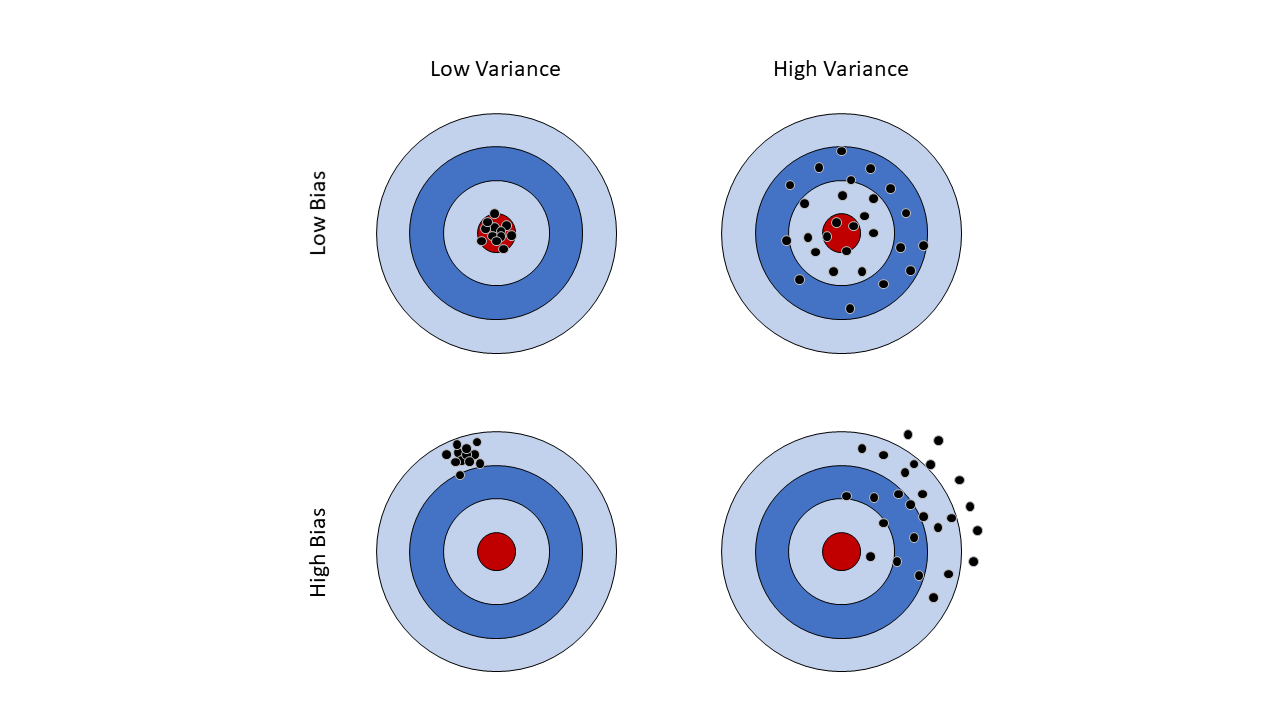
\includegraphics[scale=0.35]{biasVariabilityTargets.png}
\end{center}
\end{frame}

\begin{frame}{Bias and Variance}
\noindent\fbox{\begin{minipage}{\textwidth}
\textbf{Next step:} We want to find out how different we can expect the statistic to be from the parameter
\end{minipage}} \vspace{6mm}

There is a \textbf{big problem} when we have a \textit{biased} sample.
\begin{itemize}
    \item We often cannot quantify how the sample differs from the pop.
    \item If the sample is 'messed up,' we don't know how wrong the statistic is
    \item It is super difficult if not impossible to correct for this
\end{itemize} \vspace{6mm}

For \textbf{sampling variability} -- maybe we just do some simulations of taking a whole bunch of samples and looking at the behavior of the corresponding statistics?
\begin{itemize}
    \item We are going to give names to a few things to help us do this
\end{itemize}
\end{frame}

\begin{frame}{Review -- Distributions}
Recall that a \textbf{distribution} describes:
\begin{itemize}
    \item What values our variable can take
    \item How frequently they occur
\end{itemize} \vspace{10mm}

For the rest of today we will mostly focus on looking at quantitative variables.
\end{frame}

\begin{frame}{Population Distribution}
A \textbf{population distribution} is quite literally the distribution of a variable for the entire population
\begin{itemize}
    \item If we had complete info we could find the value for any parameter
    \item Almost always we don't \textit{actually} know what this looks like
    \item If we took a \textit{census} we could construct this
\end{itemize}
\end{frame}

\begin{frame}{Sample Distribution}
A \textbf{sample distribution} is the distribution of a variable for a single sample (data we've collected)
\begin{itemize}
    \item We can use the data to calculate statistics (ex: $\overline{x}$, s)
    \item The statistics give us an idea of how the pop. may look
\end{itemize}

\end{frame}

\begin{frame}{Sampling Distribution}
What if I actually had many samples? I could plot the distribution of all of the resulting statistics. \vspace{6mm}

A \textbf{sampling distribution} is the distribution of a whole bunch of statistics from \textit{many} samples (all with same sample size)
\begin{itemize}
    \item This will allow us to see how much the statistic itself varies from sample to sample
    \item This is a theoretical tool -- in practice we only ever take one sample
\end{itemize}
\end{frame}

\begin{frame}{Sampling Distribution}
\begin{center}
    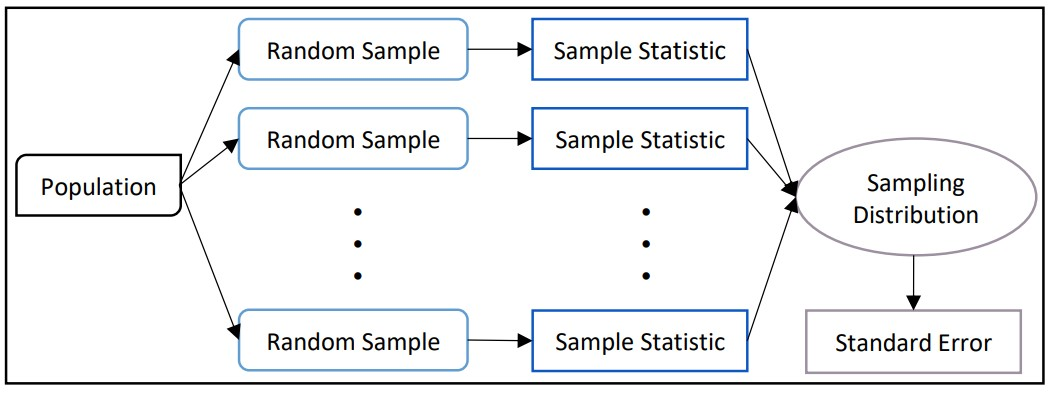
\includegraphics[scale=.6]{img/sampling_distr_method.jpg}
\end{center}
How to construct?
\begin{enumerate}
    \item Start with population.
    \item Take a sample and compute the statistic of choice
    \item Take another sample and compute the statistics
    \item Continue to take more samples and compute statistic each time
    \item Plot all of the statistics in a histogram or dotplot
\end{enumerate}
\end{frame}

\begin{frame}{Sampling Distribution}
\begin{center}
    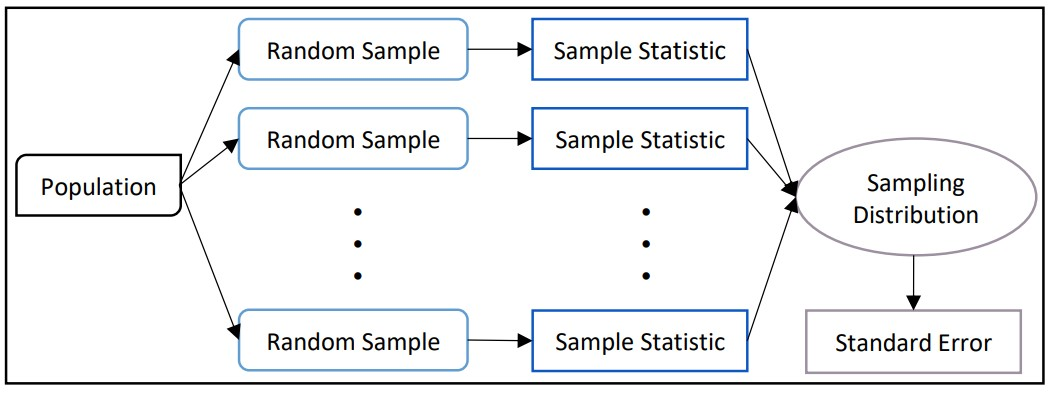
\includegraphics[scale=.5]{img/sampling_distr_method.jpg}
\end{center}
\scriptsize
\textbf{Population Variability}
\begin{itemize}
    \item Cases within the pop. vary $\rightarrow$ can describe with pop. standard deviation ($\sigma$)
\end{itemize}
\textbf{Sample Variability}
\begin{itemize}
    \item Cases within a sample vary $\rightarrow$ can describe with sample standard deviation (s)
\end{itemize} \vspace{4mm}
\textbf{Sampling Variability}
\begin{itemize}
    \item Statistics from many samples vary $\rightarrow$ describe using the std. dev. of sampling distribution
    \item \textbf{Standard Error (SE)} = std. dev. of sampling distribution
\end{itemize}
\end{frame}

\begin{frame}{Example -- Movie Budgets}
Hollywood movies released between 2012 and 2018. Recorded in millions of dollars. (n=1056)
\begin{center}
    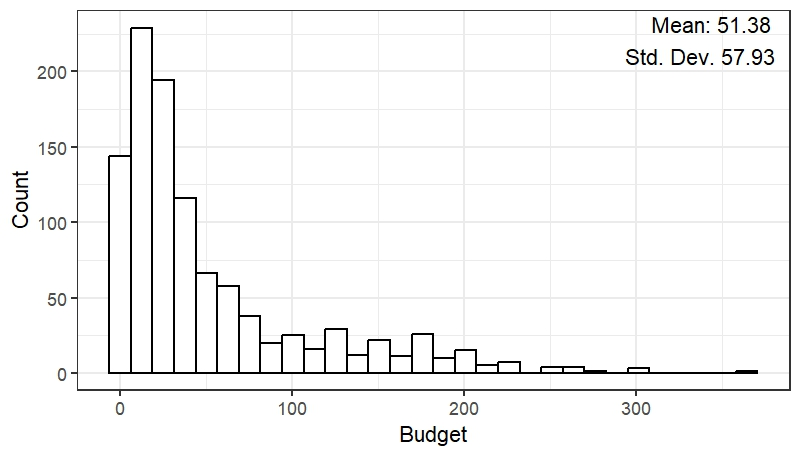
\includegraphics[scale=.7]{img/MovieBudgets_pop_distr.jpeg}
\end{center}
\end{frame}

\begin{frame}{Example -- Movie Budgets}
Sampling Distribution (sample size = 10 for each sample)
\begin{itemize}
    \item 10 samples
    \item Each dot represents the mean budget for 1 random sample
\end{itemize}
\begin{center}
    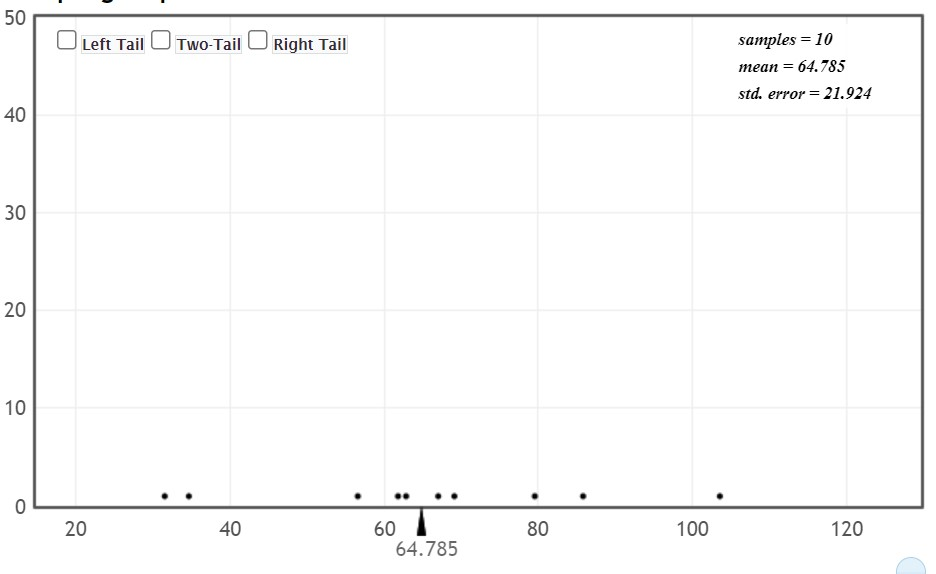
\includegraphics[scale=.55]{img/budget_dotplot1.jpg}
\end{center}
\end{frame}

\begin{frame}{Example -- Movie Budgets}
Sampling Distribution (sample size = 10 for each sample)
\begin{itemize}
    \item 1000 samples
\end{itemize}
\begin{center}
    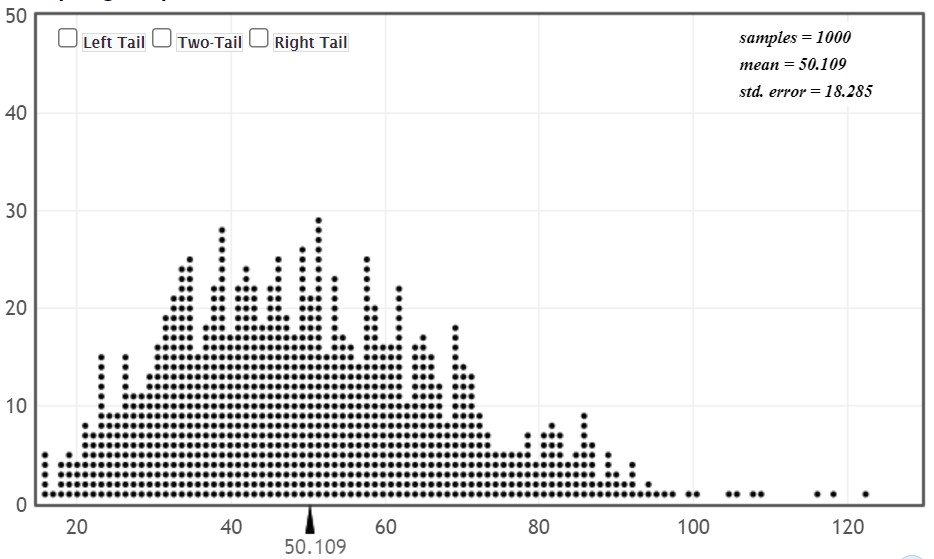
\includegraphics[scale=.55]{img/budget_dotplot2.jpg}
\end{center}
Pop: $\mu$ = 51.38
\begin{itemize}
    \item Is the sampling distribution mean similar?
\end{itemize}
\end{frame}

\begin{frame}{Sample Size}

What happens the sampling distribution when we change the sample size?

\end{frame}

\begin{frame}{Example -- Movie Budgets}
Sampling distribution (n=10 for each sample)
\begin{itemize}
    \item Shape?
    \item SE = 18.036
\end{itemize}
\begin{center}
    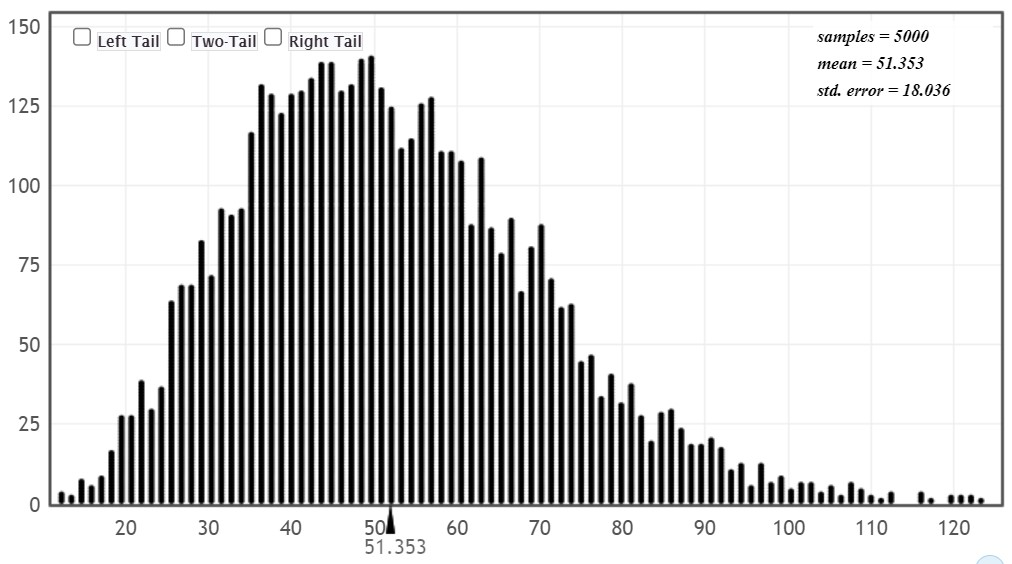
\includegraphics[scale=.6]{img/budgets_n10.jpg}
\end{center}
\end{frame}

\begin{frame}{Example -- Movie Budgets}
Sampling distribution (n=25 for each sample)
\begin{itemize}
    \item Shape?
    \item SE = 11.536
\end{itemize}
\begin{center}
    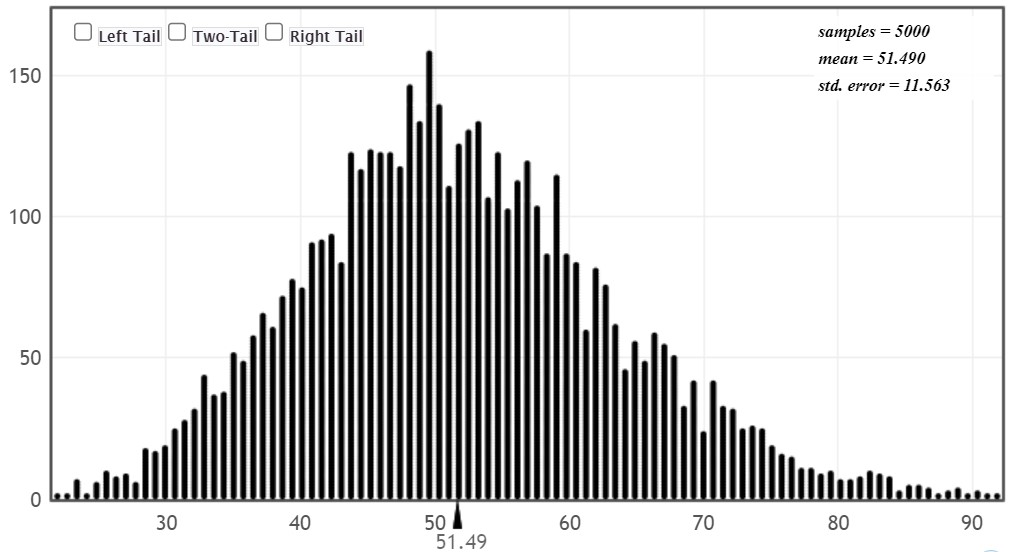
\includegraphics[scale=.6]{img/budgets_n25.jpg}
\end{center}
\end{frame}

\begin{frame}{Example -- Movie Budgets}
Sampling distribution (n=100 for each sample)
\begin{itemize}
    \item Shape?
    \item SE = 5.553
\end{itemize}
\begin{center}
    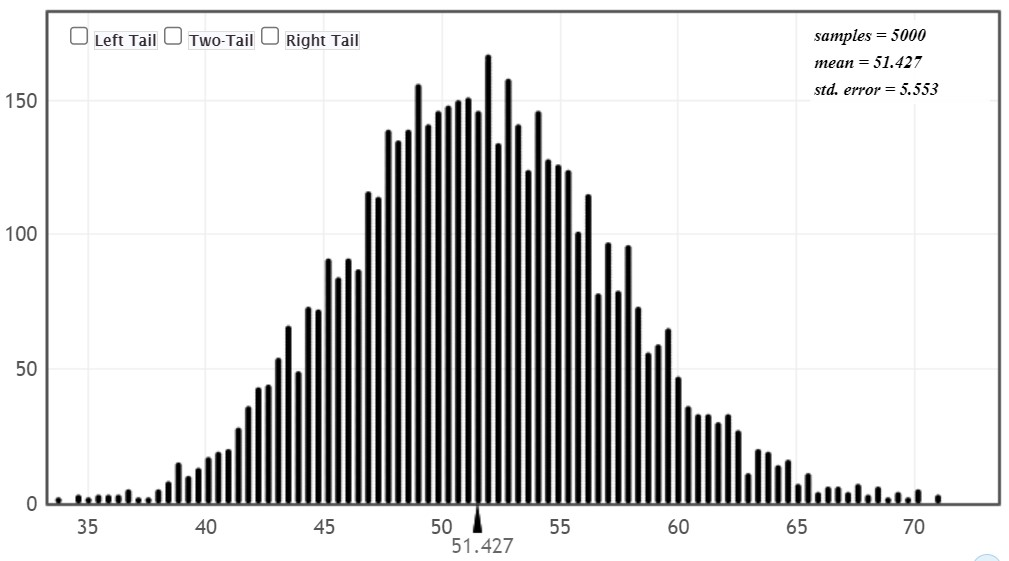
\includegraphics[scale=.6]{img/budgets_n100.jpg}
\end{center}
\end{frame}


\begin{frame}{Summary of Sampling Distributions}
\textbf{Purpose:} Sampling distributions let us see how much variability there is for our estimates (the statistics) from many samples \vspace{4mm}

\textbf{Center?}

As long as we are using \textit{random samples}, then the mean of the sampling distribution will be close to the true parameter value. \vspace{4mm}

\textbf{Shape?}

As the sample size of each sample increases:
\begin{itemize}
    \item the distribution becomes more and more bell-shaped
\end{itemize} \vspace{4mm}

\textbf{Standard Error (SE)} -- variability of statistics from our many samples

As the sample size of each sample increases:
\begin{itemize}
    \item The standard error of the sampling distribution decreases
    \item our estimates become more \textit{precise}
\end{itemize}
\end{frame}

\begin{frame}{Next Time}
We are going to keep working with sampling distributions. \vspace{5mm}

We will use Standard Error to help us quantify how far off we think our estimates might be. \vspace{5mm}

We can use sampling distributions for all kinds of statistics like medians, proportions, correlations (not just means)
\end{frame}

\begin{frame}{Check Your Understanding}
\begin{itemize}
    \item What does \textbf{Inference} mean?
    \item What was the purpose of constructing sampling distributions in terms of estimation?
    \item How does sample size affect sampling distributions?
\end{itemize}
\end{frame}

%%%%%%%%%%%%%%%%

%\begin{frame}
%\begin{columns}
%
%  \begin{column}{0.45\textwidth}
%%
%  \end{column}
%  \begin{column}{0.45\textwidth}
%%
%  \end{column}
%
%\end{columns}
%\end{frame}


\end{document}

